\documentclass{article}
\usepackage[utf8]{inputenc}
\usepackage{geometry} 
\geometry{a4paper}  
%\usepackage[parfill]{parskip} 
\usepackage{graphicx}	
\usepackage{amsmath}
\usepackage{fullpage}
\usepackage{setspace} 
\usepackage{lineno}
\usepackage[none]{hyphenat}
\usepackage{listings}

\usepackage[round]{natbib}	

\title{Reproducible, flexible and high throughput data extraction from primary literature: The metaDigitise R package}
\author{Joel L. Pick, Shinichi Nakagawa \& Daniel W.A. Noble}
% \date{}

\begin{document}
\doublespacing
%\raggedright

\maketitle
Prepared for: Journal of Statistical Software

\section*{Abstract}

Keywords: meta-analysis, comparative analysis, data extraction, R, reproducibility, figures, images, summary statistics

\clearpage
\section*{Introduction}

Meta-analysis is becoming increasingly common in many research fields. They make use of various summary statistics from studies to generate effect size estimates and their sampling error variance to understand whether particular experimental manipulations, or relationships between variables, show strong overall effects and attempt to explain variation among these effects (Nakagawa et al. 2017). Meta-analysis relies foremost on data extracted from primary literature – more specifically statistics that have been reported in the text or tables of research papers. However, necessary summary statistics are often presented in figures, and so, these need to be manually extracted using digitsiing programs to be used in the final analysis. Although there are several existing tools to perform tasks like this, these tools are not made for this specific purpose (i.e. a meta-analysis). Specifically, they do not differentiate between common plot types that are use to present data, meaning that they require a large amount of downstream data manipulation. For example, extracting often only provides the raw data or values from plots. This means that these data need to be imported into other programs to calculate correlations (if scatter plots) or errors on means (from mean error plots) need to be back calculated by hand to convert them to a common type (e.g., standard errors to standard deviations). Digitising programs often do not allow for different grouping of points to be made, and frequently do not integrate metadata (such as variable names, group names and sample sizes) at the time of data extraction. Additionally, existing stand-alone software does not allow easy import into commonly used statistical software (such as R), or try to optimize the research pipelines to facilitate editing and reproducibility. These are major issues because extracting from figures can be an incredibly time-consuming process. Furthermore, meta-analyses can have a major impact on research fields, and should be expanded upon as more research comes to light. Having a tool that facilitates reproducibility in meta-analyses will increase transparency and go a long way to resolving the reproducibility crises we are seeing in many fields.

Here, we present an interactive R package, `metaDigitise`, which is designed for large scale data extraction from figures, specifically catering to the the needs of meta-analysts. To this end, we provide tools specific to data extraction from common plot types (mean and error plots, box plots, scatter plots and histograms, see Figure \ref{fig:plot_type}). `metaDigitise` operates within the R environment making data extraction, analysis and export more streamlined. It also provides users with options to conduct the necessary calculations on raw data immediately after extraction so that comparable summary statistics can be obtained quickly. Summaries will condense multiple figures into data frames or lists (depending on the type of figures) and these objects can easily be exported from R, or if using the raw data, analysed in any way the user desires. Conveniently, when needing to process many figures at different times `metaDigitise` will only import figures not already completed within a directory. This makes it easy to add new figures at anytime. `metaDigitise` has also been built for reproducibility in mind. It has functions that allow users to redraw their digitisations on figures, correct anything and access the raw calibration data which is written automatically for each figure that is digitised into a special folder within the directory. This makes sharing figure digitisation and reproducing the work of others simple and easy, and allows meta-analysts to update meta-analyses more easily.


\begin{figure}[ht] 
%\onehalfspacing
 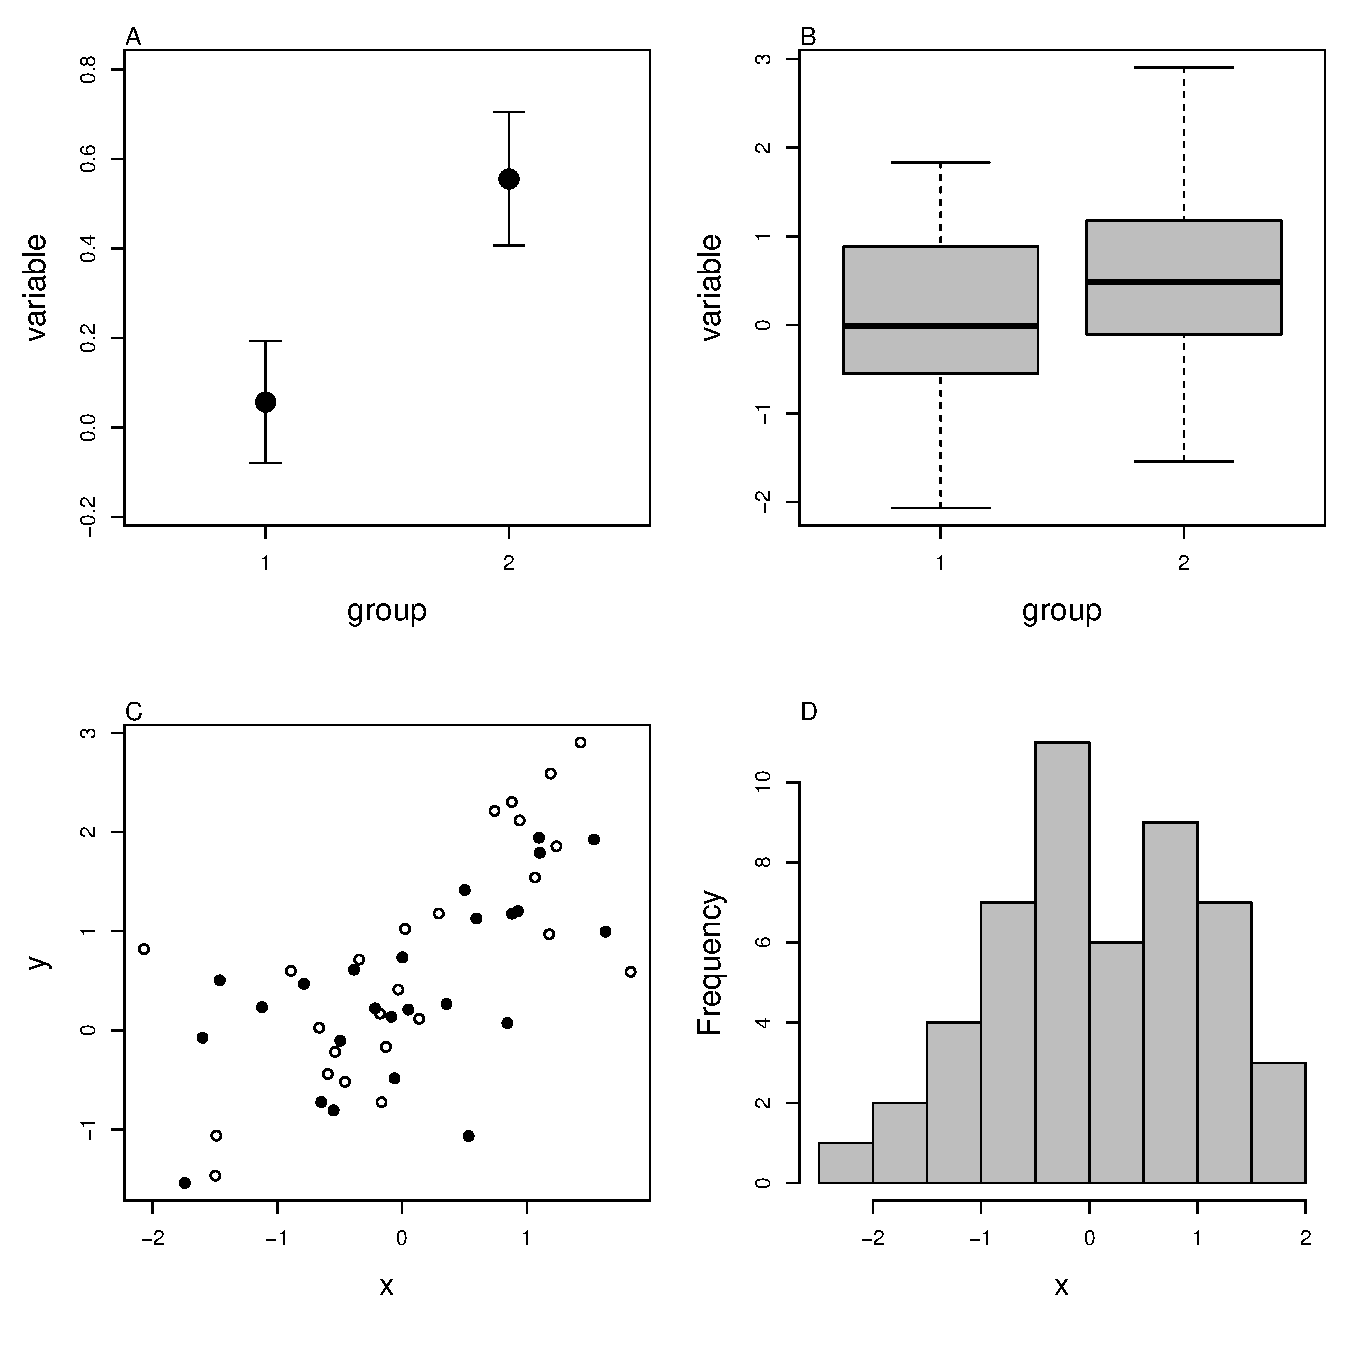
\includegraphics[width=0.9\textwidth]{fig_plot_type.pdf} 
 \caption{Four plot types that metaDigitise is designed to extract data from: A) mean and error plot, B) box plot, C) scatter plot and D) histogram. Data is taken from the iris dataset in R. A and B are plotted with the whole dataset, C and D are just the data for the species setosa.}
\label{fig:plot_type}
\end{figure}

\section*{Directory Structure and Reproducibility}

The `metaDigitise` package is quite flexible. There is one main function in the package, metaDigitise, which interactively takes the user through the process of extracting figures from graphs. `metaDigitise` can work on a directory with figures (currently .png, .jpg, .tiff, .pdf images can be used) from many different papers and that are of different types (see below). However, users can get creative in how they set up the directories of figures to facilitate extraction. For example, one might have 3–4 figures from a single paper that need extracting and the user may want to focus on a single paper at a time while the information about a paper is on hand. This could be done by simply setting up a file structure as follows and then using `metaDigitise` with path names (i.e., directory) for each papers folder:

\begin{lstlisting}
	* Main project directory
		+ Paper1_P1
			+ Figure1.png
			+ Figure2.png
			+ Figure3.png
		+ Paper2_P2
			+ Figure1.png
			+ Figure2.png
			+ Figure3.png
\end{lstlisting}

An alternative directory structure (and probably the most flexible) would be to simply have a set of different figures with an informative and relevant naming scheme to make it easy to identify the paper and figure the data come from. This cuts out the need to change directories constantly. For example the directory structure could look like:

\begin{lstlisting}
	* Main project directory
		+ FiguresToExtract
			+ P1_Figure1_trait1.png
			+ P1_Figure2_trait2.png
			+ P1_Figure3_trait3.png
			+ P2_Figure1_trait1.png
			+ P2_Figure2_trait2.png
			+ P2_Figure3_trait3.png
\end{lstlisting}

The above directory structure is probably the easiest in combination with a clear and unambiguous naming scheme for each figure. Even if only figures from a single paper are digitised, one paper at a time, an overall figure directory will work perfectly because `metaDigitise` will only cycle through incomplete figures, so figures can be added at anytime. 

Nonetheless, how users set up their directory is really up to them. However, it is important for users to think carefully about reproducibility at this stage. Would they like to share the entire project folder with colleagues? or would they prefer to simply share the image folder? The answers to these questions are important because relative path names are stored in `metaDigitise` objects, meaning that the directory structure (currently at least) needs to be the same for colleagues to re-load previously digitised objects. Therefore, the working directory needs to be set to either the "main project directory" or the "FiguresToExtract" directory and relative path names (e.g., users should specify dir = "./FiguresToExtract/" if setting the working directory to "Main project directory") used as opposed to absolute paths. This facilitates reproducibility should colleagues want to see the digitisations or integrate previously digitised figures with newly digitised figures. All users need to provide them with is the project or image folder.

\section*{High-throughput Digitisation of Figure(s) within a Directory}
metaDigitise was created with the idea that the user would likely have multiple images to extract from. It therefore operates in the same way whether the user has one or multiple images. It assumes that the user has put all the figures needed for extraction in one parent directory (see above). Users can extract single figures (if this is all they have) using the `metaDigitise` function with a path name to the directory with the file. However, often many figures need extracting from a single paper or set of papers. `metaDigitise` will also handle these situations seamlessly by simply cycling through all figures within a directory. This is useful because it expedites digitising figures by preventing users from having to constantly change directories and / or open new images. It operates by recognizing all the figures in a folder and bringing up each figure automatically allowing the user to click and enter relevant information about a figure as they go. All this information is then stored in a data frame or list at the end of the process, saving quite a bit of time. Users can stop mid-way through a folder by simply exiting after the last plot they have digitised. The data from completed figures will automatically be written to a special `caldat/` folder that is created when first executing the metaDigitise function. Digitised data along with metadata for figures are stored in caldat/ for later use and editing (see below)

In order to correctly extract data from figures metaDigitise always requires the user to calibrate the axes in the figure. To do this, the user is required to click on two known points on the axis in question, and then enter the value of those points in the figure (Figure \ref{fig:calibrate}). Using this information, metaDigitise then calculates the value of any clicked points in terms of the figure axes. In the case of mean and error plots and box plots, it calibrates only the y axis (assuming the x axis is redundant). For scatter plots and histograms both axes are calibrated.

\begin{figure}[!h] 
%\onehalfspacing
 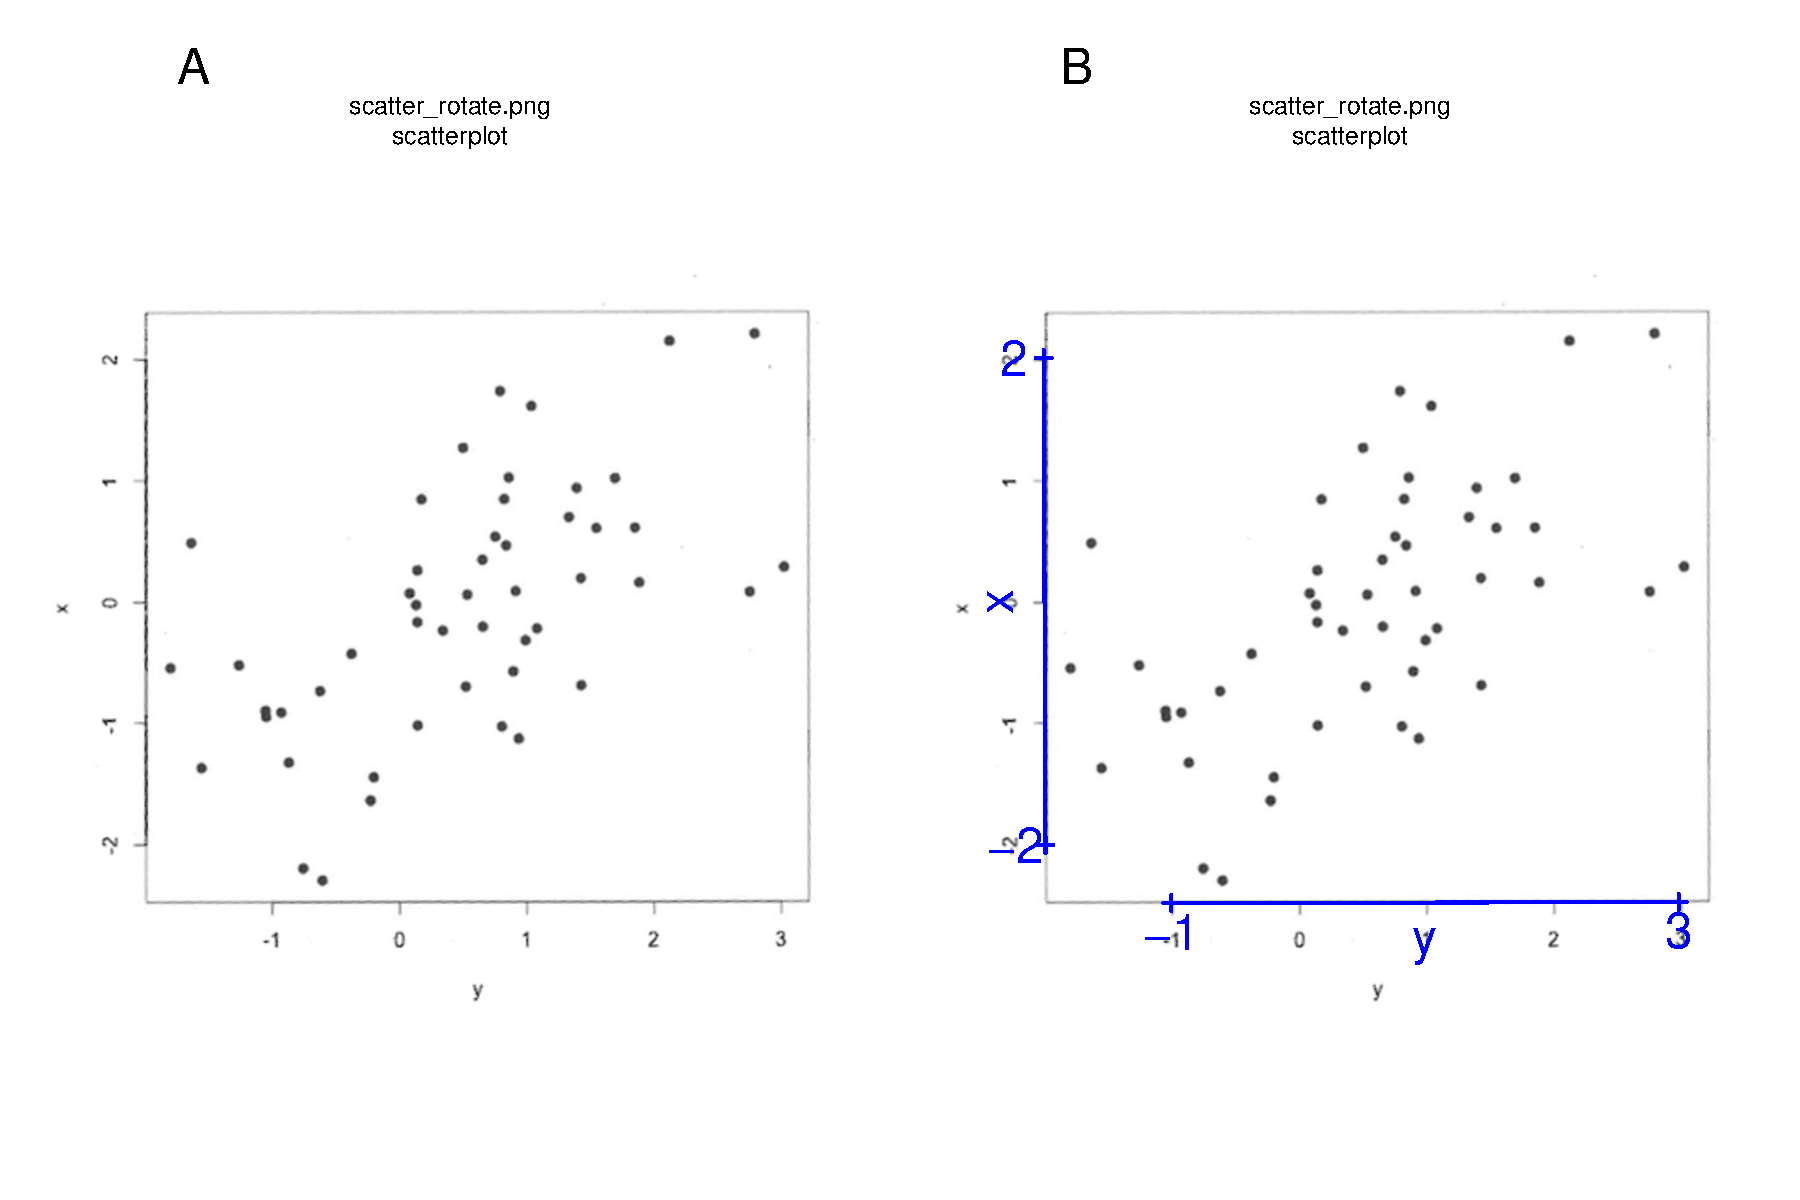
\includegraphics[width=0.9\textwidth]{fig_calibrate.pdf} 
 \caption{Axis calibration. The user defines two points on each axis and labels them according to the values shown in the figure.}
\label{fig:calibrate}
\end{figure}

A particularly powerful and flexible aspect of metaDigitise is its ability to recognize figures that are not already completed and only bring up those figures that have not been digitised in subsequent calls of the function. This means that new figures can be added at any time as the project develops and previously digitised figures are simply ignore during processing, but their data re-integrated within the final output after new files are completed. 

From all plot types, metaDigitise summarises the data from a figure or set of figures as a mean, standard deviation and sample size, for each identified group within the plot (should multiple groups exist). These are the summary statistics needed to create many of the relevant effect sizes and sampling error for a meta-analysis. In the case of scatter plots, metaDigitise also returns the correlation coefficient between the points within each identified group. 

\subsection{Diverse Plot Types}
metaDigitise recognises four main types of plot; Mean and error plots, box plots, scatter plots and histograms, shown in Figure \ref{fig:plot_type}. Each of these can be processed together and integrated into a single output. Alternatively, users can keep like figures together and process them separately.

%%% Equations for mean and sd
%% pooled stats: 
% \begin{align}
% \mu _{X}&={\frac {\sum _{i}{N_{X_{i}}\mu _{X_{i}}}}{\sum _{i}{N_{X_{i}}}}}
% \\
% \sigma _{X}&={\sqrt {{\frac {1}{\sum _{i}{N_{X_{i}}-1}}}\left(\sum _{i}{\left[(N_{X_{i}}-1)\sigma _{X_{i}}^{2}+N_{X_{i}}\mu _{X_{i}}^{2}\right]}-\left[\sum _{i}{N_{X_{i}}}\right]\mu _{X}^{2}\right)}}
% \end{align}


\begin{figure}[!h] 
%\onehalfspacing
 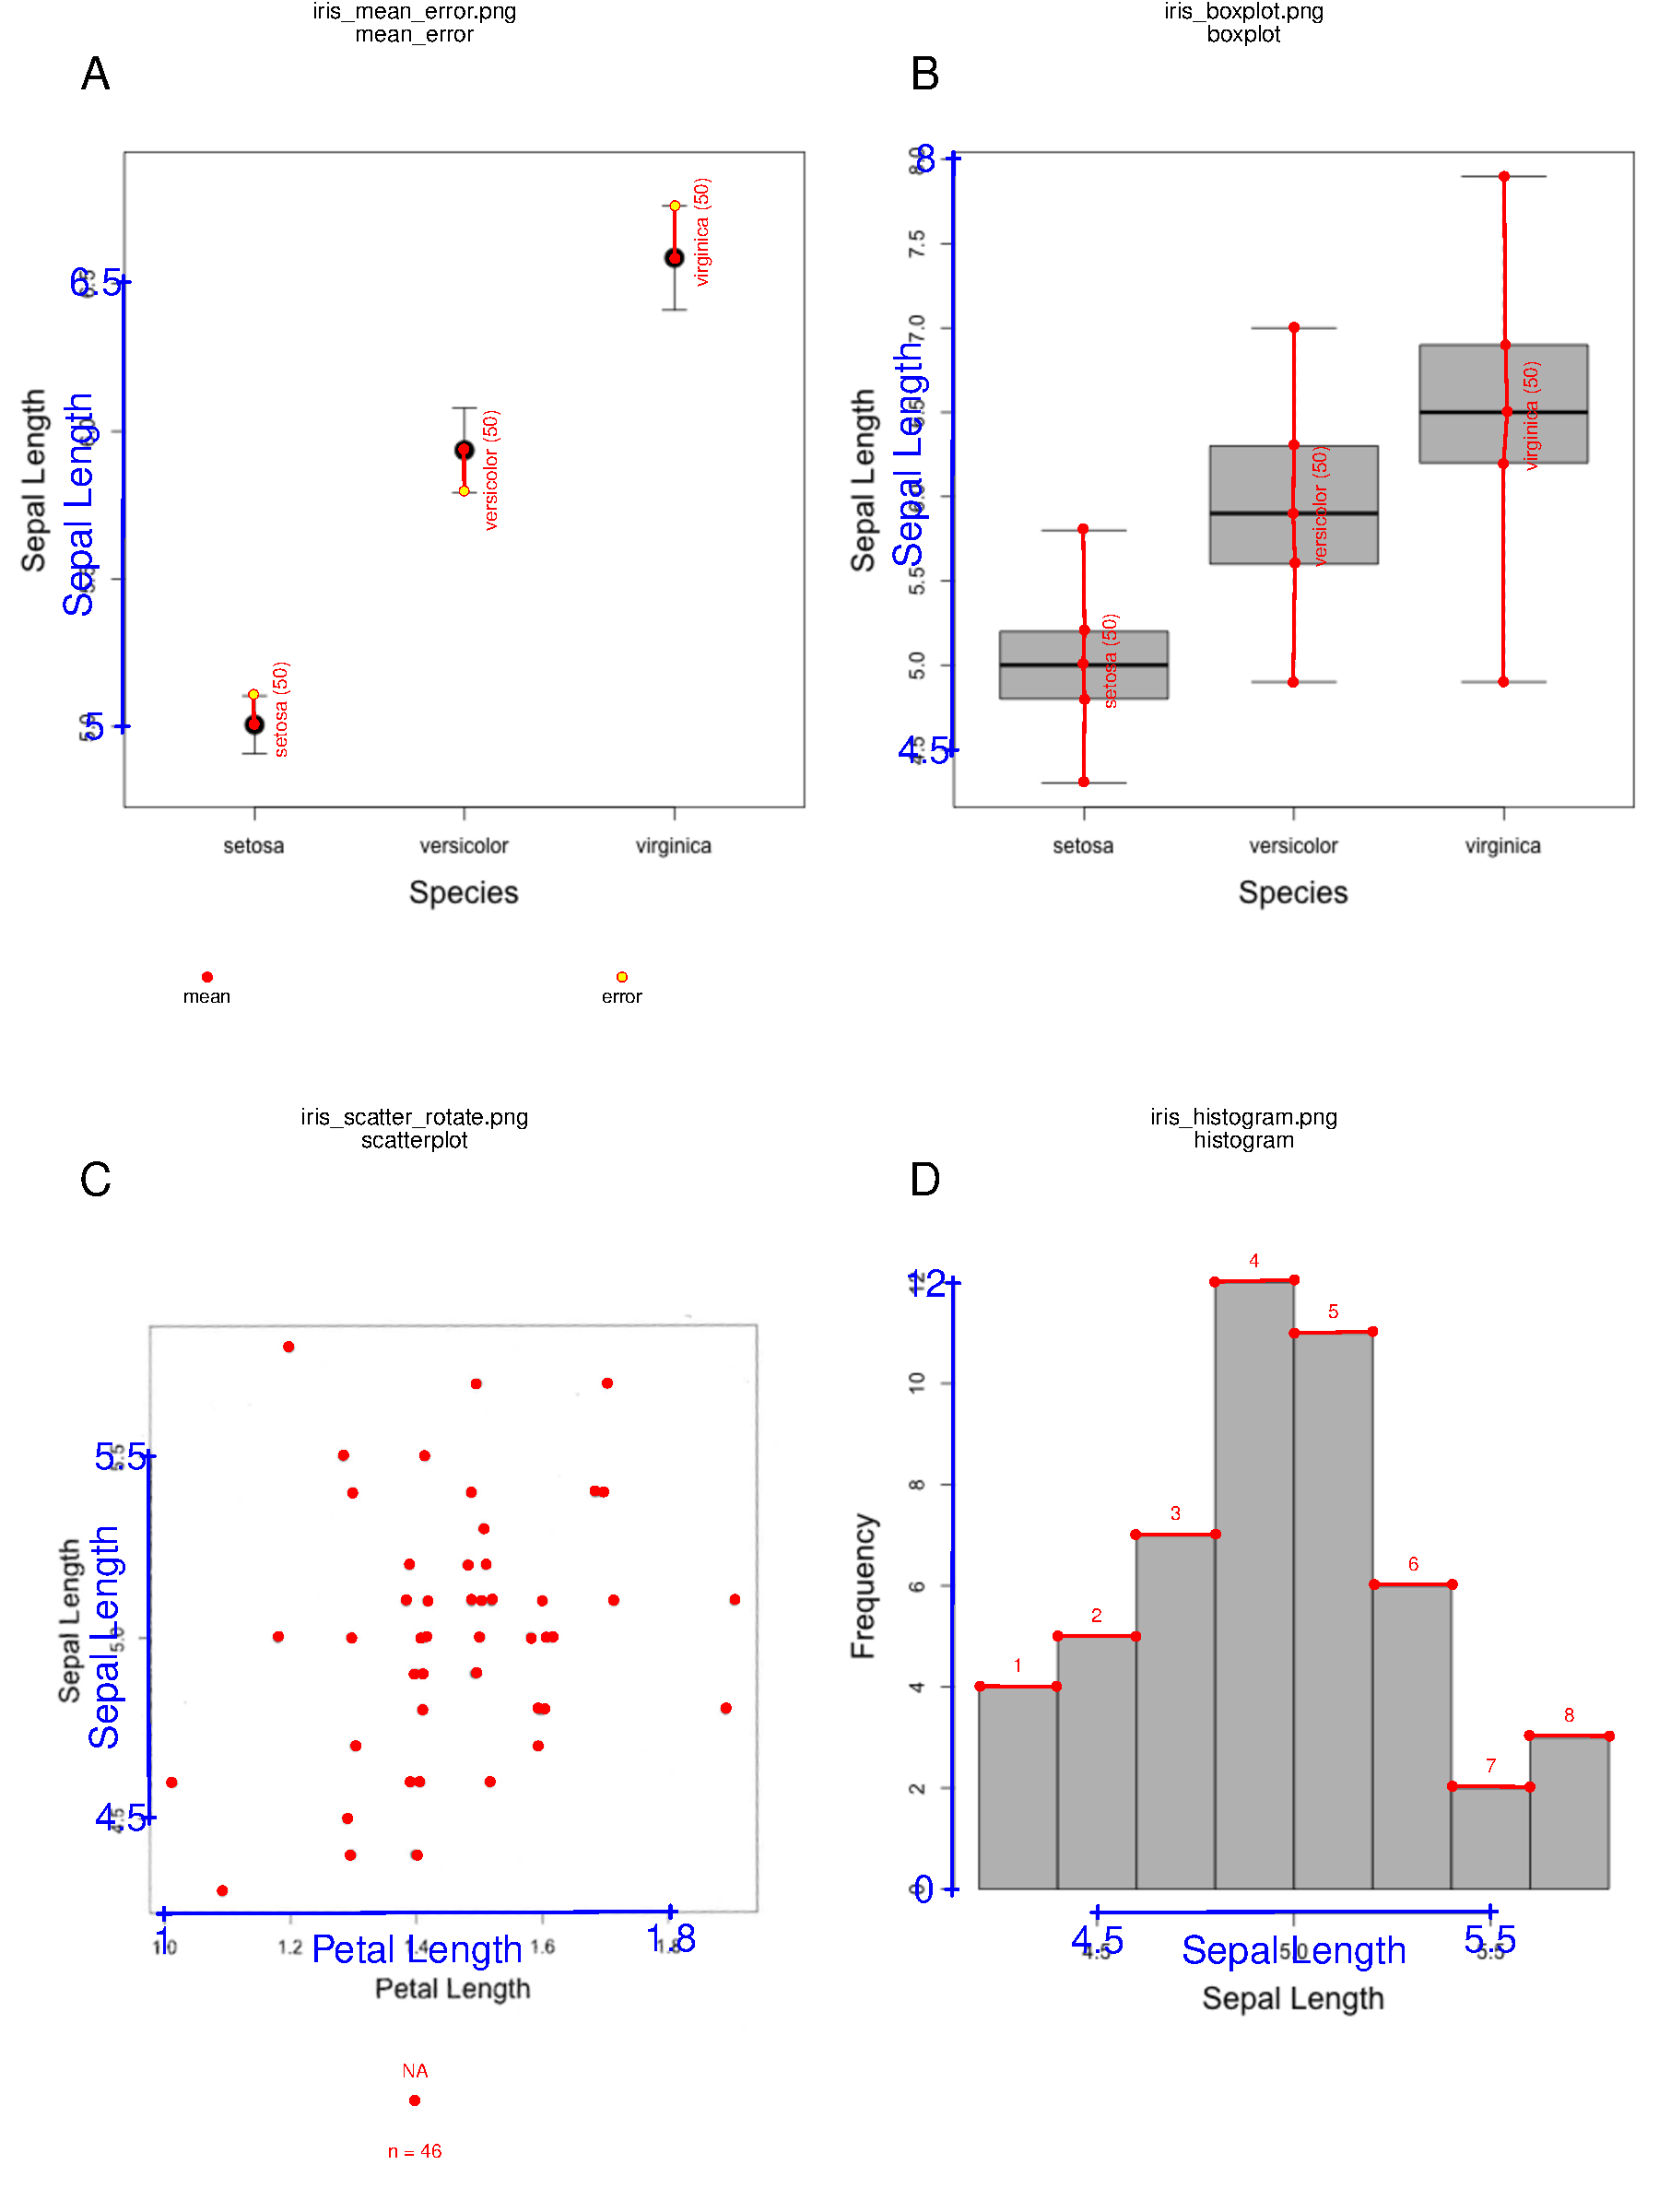
\includegraphics[width=0.9\textwidth]{fig_all_extract.pdf} 
 \caption{Demonstration of data extraction from different plot types}
\label{fig:all_extract}
\end{figure}

\subsubsection{Mean and error plots} 
metaDigitise prompts the user to enter groups names and allows the user to enter sample sizes, which are used in downstream processing. The user is then prompted to click on an error bar followed by the mean. Error bars above or below the mean can be clicked - sometimes one is clearer than the other. metaDigitise assumes that the error bars are symmetrical. Where the user has clicked the error is displayed in a different colour to the mean (Figure \ref{fig:all_extract}A). The user can subsequently add more groups or remove groups.

\subsubsection{Box plots}
 metaDigitise prompts the user to enter groups names and allows the user to enter sample sizes, which are used in downstream processing. The user is then prompted to click on the maximum, upper quartile, median, lower quartile and minimum. metaDigitise will check that the maximum is greater than the minimum, and return an warning if that is not the case. The user can subsequently add more groups or remove groups.

\subsubsection{Scatter plots}
 metaDigitise prompts the user to enter groups names and then to click on points. Points added by mistake can be deleted. The user can subsequently add groups, edit groups (add or remove points) or delete groups. Different groups are plotted in different colours and shapes, with a legend at the bottom of the figure (Figure \ref{fig:all_extract}C). The x and y coordinates are returned.

\subsubsection{Histograms}
metaDigitise prompts the user to enter groups names and then to click on the top corners of each bar. bars can subsequently be deleted. MetaDigitise then calculates the midpoint and the frequency for each bar. 

\subsection{Re-importing, Editing and Plotting Previously Digitised data}

A particularly useful feature of `metaDigitise` is its ability to re-import, edit and re-plot previously digitised figures. Running metaDigitise brings up a series of prompts for the user using a main menu that provides access to a number of its features: 

\begin{verbatim}
	Do you want to...
1: Process new images
2: Import existing data
3: Edit existing data
Selection: 
\end{verbatim}

The user simply enters in the numeric value that corresponds to what they would like to do. Choosing "Process new images" will permit users to digitise new figures, integrating previously completed digitisations along with newly digitised data together at the end of the session, or when the user decides to quit. If the user chooses "Import existing data", they have the option of either 1) importing all data or 2) importing a particular figure that has been digitised. If 2, then a list of files are provided to the user that they can select. 

Editing existing data allows users to easily re-plot or edit information or digitisations that have previously be done for any plot. This is accomplished by guiding the user through a new set of options:

\begin{verbatim}
Choose how you want to edit files:
1: Cycle through images
2: Choose specific file to edit
3: Enter previously omitted sample sizes
Selection: 
\end{verbatim}

If the user is unsure about the name of the specific figure they need to edit or simply want to just check the digitisations of figures they can choose "Cycle through images", which will bring up each figure, one by one, overlaying the calibrations, group names (if they exist), sample sizes (if they were entered) and the selected points. Alternatively, choosing option 2, will bring up a list of the completed files in the folder and the specific file can be chosen, at which point it will be replotted. Either of these options will cycle through a number of questions asking the user what they would like to edit:

\begin{verbatim}
Edit rotation? If yes, then the whole extraction will be redone (y/n) n
Change plot type? If yes, then the whole extraction will be redone (y/n) n
Variable entered as: Sepal length
Rename Variables (y/n) n
Edit calibration? (y/n) n
Re-extract data (y/n) y
Change group identifier? (y/n) n
Add group, Delete group or Finish plot? a/d/f d
1: setosa
2: versicolor
3: viriginica
Selection: 2
Add group, Delete group or Finish plot? a/d/f a
\end{verbatim}

A whole host of information can be edited from the rotation, plot type, the variable name that was provided, the calibration and even the digitisation of groups. When editing the metaDigitise object is re-written to the caldat folder and the edits are immediately integrated into the existing object once complete. 

\section{Additional Features}

\subsection{Figure Rotation and Adjustment}
Figure may have been extracted from old publications, for example from scanned images, and so are not perfectly orientated on the image. This will make the calibration of the points in the figure from the image problematic. metaDigitise allows users to rotate the image. By clicking two points on the x-axis, metaDigitse calculates the angle needed to rotate the image so the x-axis is horizontal, and rotates it. (Figure \ref{fig:rotate}A,B)

\begin{figure}[!h] 
%\onehalfspacing
 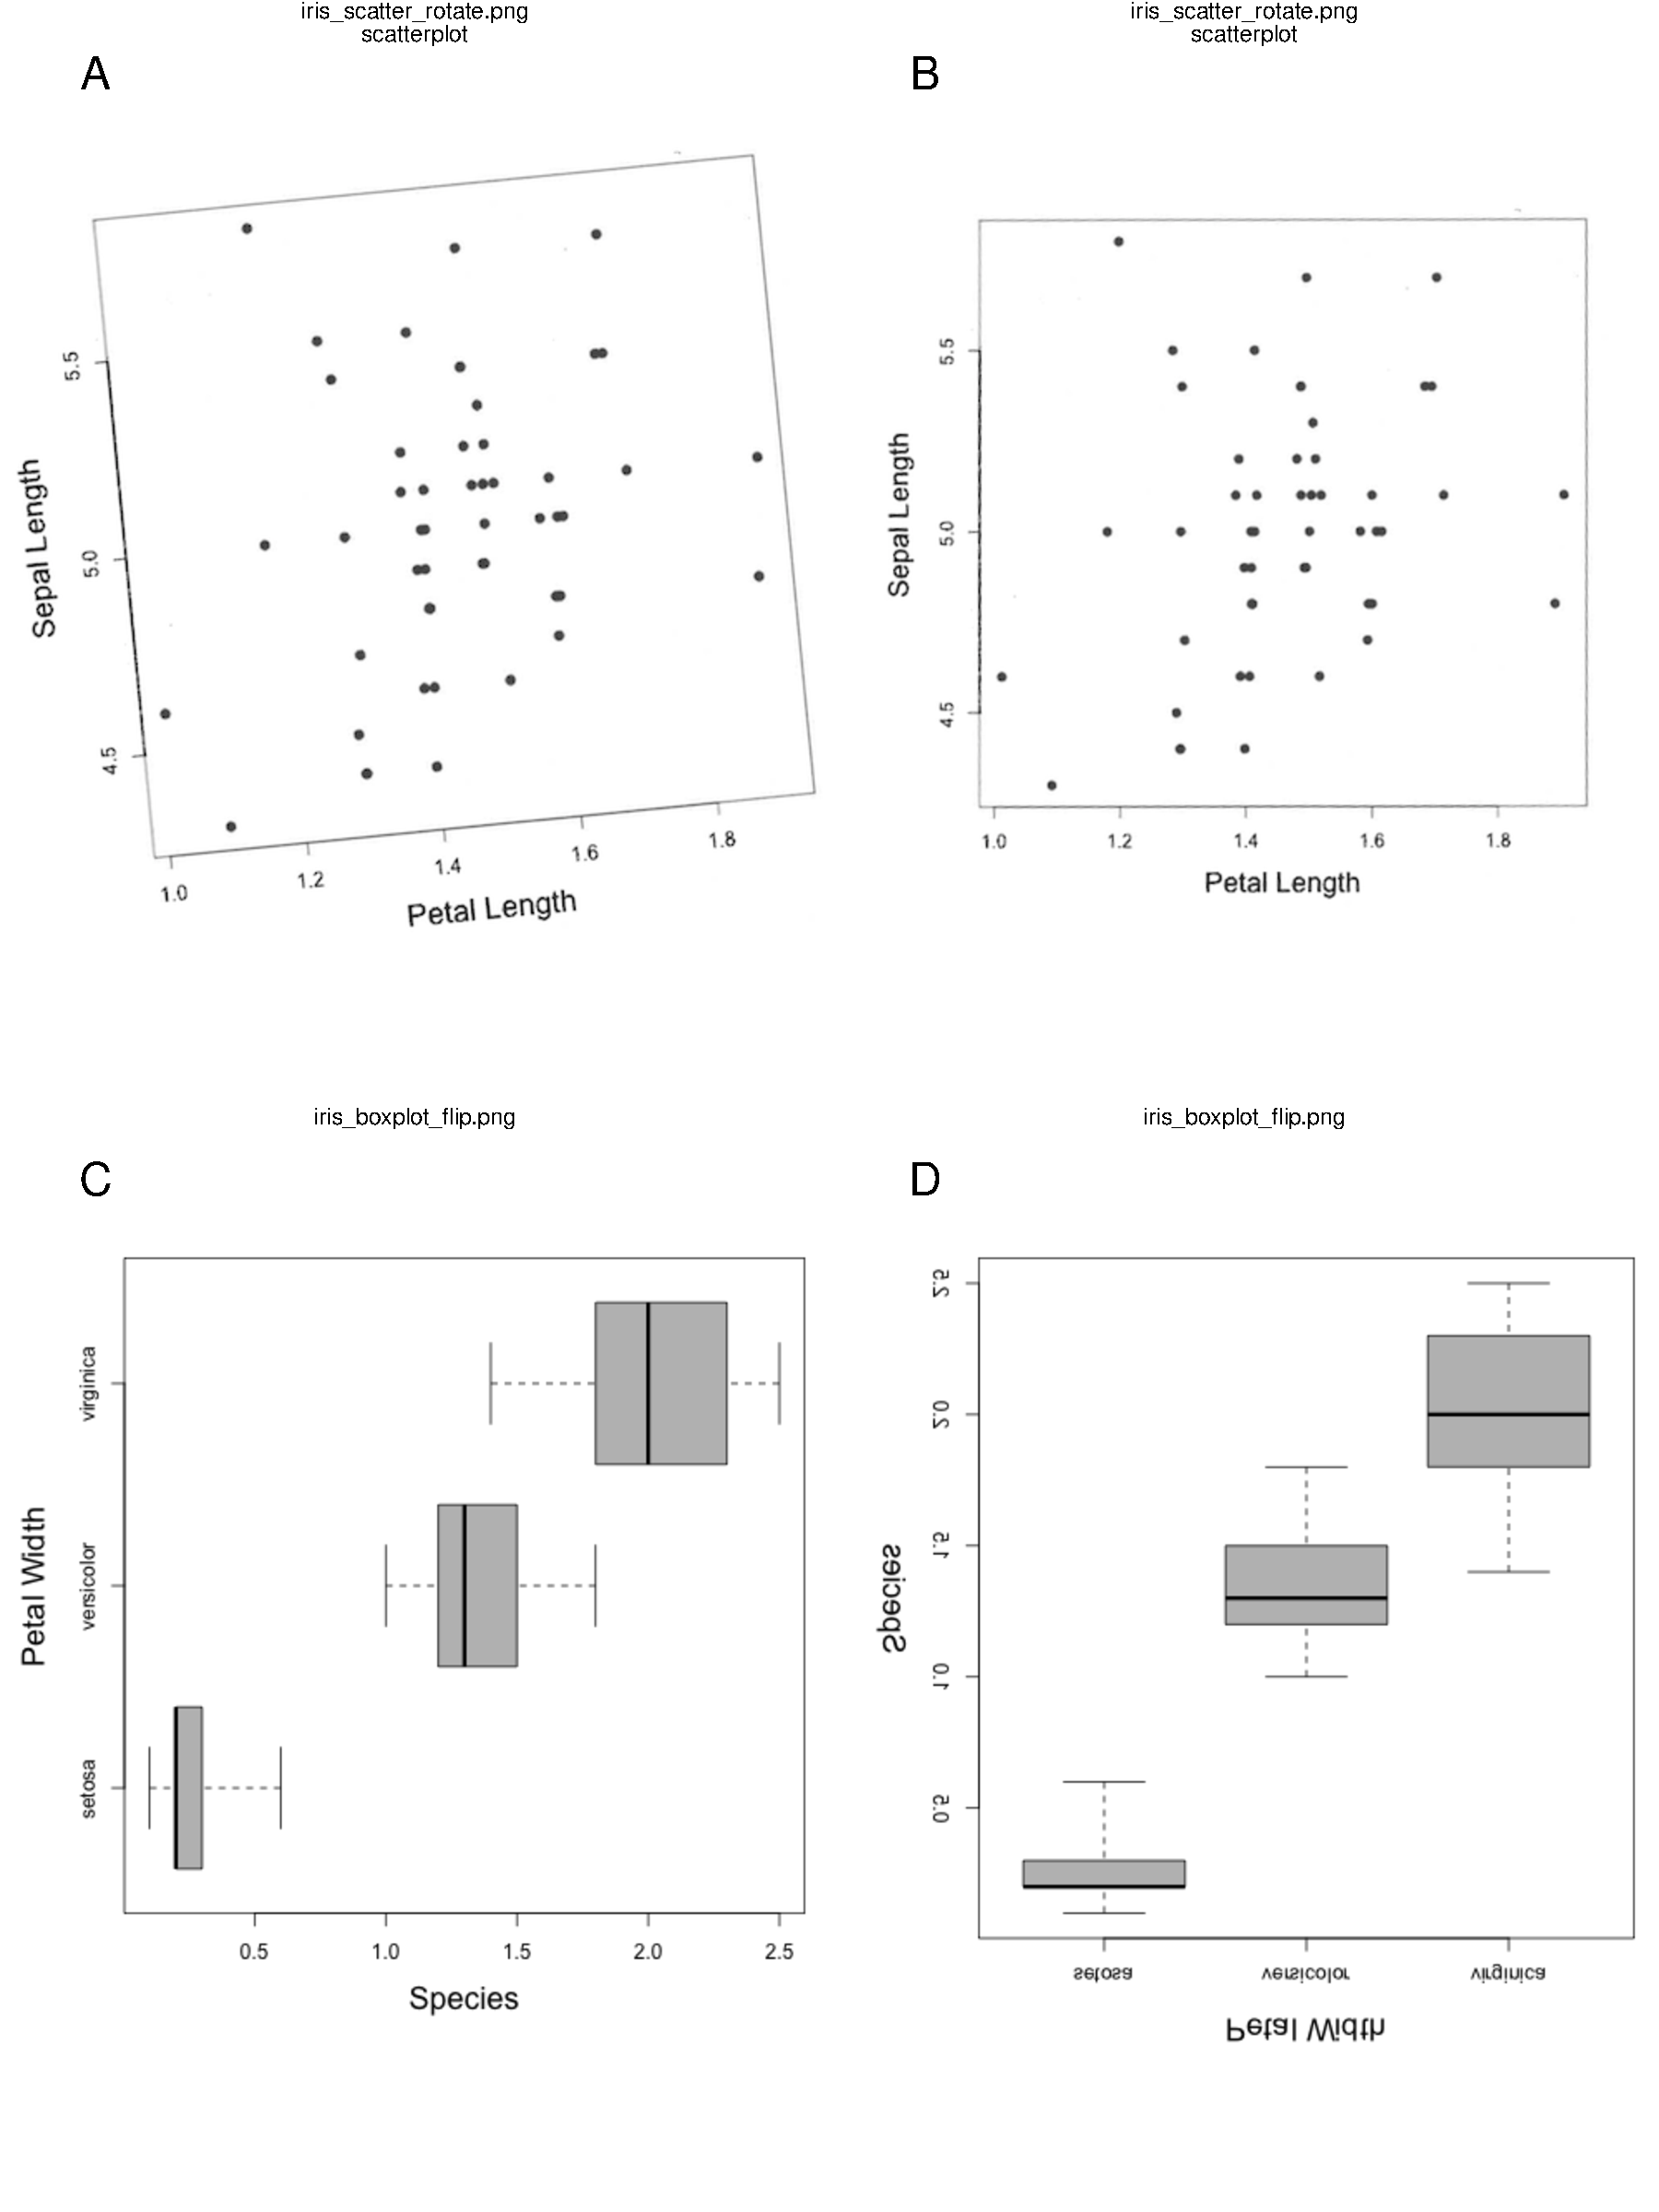
\includegraphics[width=0.9\textwidth]{fig_rotate.pdf} 
 \caption{Figure rotation. A) and B) show how non-aligned imaged can be realigned through user defined rotation. C) and D) show show figures can be re-orientated so as to aid data input.}
\label{fig:rotate}
\end{figure}

Furthermore, in some figures mean and error, boxplots or histograms may be presented with horizontal bars. metaDigitise assumes that the bars are vertical, but allows the user to flip the image so that the bars are vertical (Figure \ref{fig:rotate}C,D).

\subsection{Obtaining Raw Data}

While metaDigitise provides users with the summary statistics by default, for all plot types, in many cases the user may actually be interested in obtaining the raw digitised data from scatter plots. This is very easy to do my changing the default `summary` argument from TRUE to FALSE in the metaDigitise function. Instead of providing the user with summary statistics it will return a list containing four slots for each of the figure types (mean error, box plot, histogram and scatter plots). An example of a data object returned from digitising figures is as follows:

\begin{verbatim}
str(data)
List of 3
 $ mean_error :List of 1
  ..$ 002_Doe_2013_Fig1.png:'data.frame': 3 obs. of  5 variables:
  .. ..$ id      : Factor w/ 3 levels "setosa","versicolor",..: 1 2 3
  .. ..$ mean    : num [1:3] 5 5.93 6.59
  .. ..$ error   : num [1:3] 0.111 0.148 0.178
  .. ..$ n       : num [1:3] 50 50 50
  .. ..$ variable: chr [1:3] "Sepal length" "Sepal length" "Sepal length"
 $ hist       :List of 1
  ..$ 003_Doe_2013_Fig3.png:'data.frame': 8 obs. of  3 variables:
  .. ..$ midpoints: num [1:8] 4.3 4.5 4.7 4.9 5.1 ...
  .. ..$ frequency: num [1:8] 4 5 7 12 11 6 2 3
  .. ..$ variable : chr [1:8] "Sepal length" "Sepal length" "Sepal length" "Sepal length" ...
 $ scatterplot:List of 1
  ..$ 001_Anderson_1935_Fig1.png:'data.frame':  83 obs. of  8 variables:
  .. ..$ id        : Factor w/ 2 levels "setosa","versicolor": 1 1 1 1 1 1 1 1 1 1 ...
  .. ..$ x         : num [1:83] 2.3 2.9 3 3 3 ...
  .. ..$ y         : num [1:83] 4.5 4.4 4.41 4.3 4.8 ...
  .. ..$ group     : num [1:83] 1 1 1 1 1 1 1 1 1 1 ...
  .. ..$ col       : Factor w/ 2 levels "red","green": 1 1 1 1 1 1 1 1 1 1 ...
  .. ..$ pch       : num [1:83] 19 19 19 19 19 19 19 19 19 19 ...
  .. ..$ y_variable: chr [1:83] "Sepal length (mm)" "Sepal length (mm)" "Sepal length (mm)" "Sepal length (mm)" ...
  .. ..$ x_variable: chr [1:83] "Sepal width (mm)" "Sepal width (mm)" "Sepal width (mm)" "Sepal width (mm)" ...
\end{verbatim}

Here, the user can easily access the list of raw scatter plot data by simply extracting the scatter plot slot:

\begin{verbatim}
scatterplot <- data$scatterplot
\end{verbatim}

%check extraction
%Including addition of N later

\section{Example}
%% scatterplot from airquality data
We'll now turn to an example of how metaDigitise works using figures generated using the well known iris data set \ref{fig:all_extract}. Users can install metaDigitise from GitHub as follows:

\begin{verbatim}
	install.packages("devtools")
	devtools::install_github("daniel1noble/metaDigitise")
	library(metaDigitise)
\end{verbatim}

Assume that we have three figures, from two hypothetical studies, that we would like to extract summary statistics from. Each hypothetical study quantifies sepal length and width on a number of iris species. 

It then prompts the user to select whether they want to extract from new images, import previously extracted data or edit previously extracted data. Extracting from new images takes the user through the steps outlined below, figure by figure, giving the user the option to quit the process after each figure. If this process has already been started when the user starts metaDigitise, then it starts where the user left off. Similarly if the user adds new images to the parent directory after all other images are extracted (or part way through), the new images will be integrated into the extraction procedure. After extraction (or upon quitting the function), the extracted data will be returned. %% explain summary etc

\section{Testing}
%% simulated data
%% x people doing y plots

\end{document}

